\documentclass{article}
\usepackage{graphicx}

\usepackage{tikz}


\usepackage{pgfplots}

\definecolor{cornflower}{rgb}{0.12549, 0.29020, 0.52941}
\def\width{18}

\begin{document}
	\begin{center}
		\begin{tikzpicture}[scale=2]
		\node[anchor=south west,inner sep=0] at (0,0) {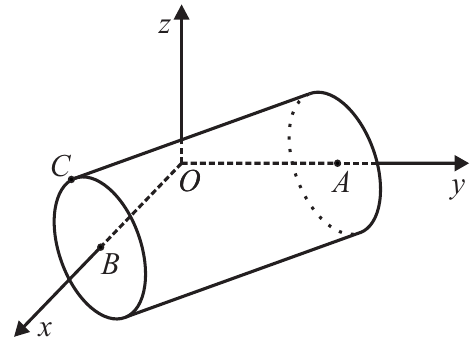
\includegraphics[width=\linewidth]{ex5.png}};
		
		\draw [cornflower!30,step=0.1,thin] (0,0) grid (6.2,4.5);
		\draw [cornflower,step=0.5,thin] (0,0) grid (6.2,4.5);
		
		\coordinate (A) at (4.335, 2.35);
		\coordinate (B) at (1.3, 1.257);
		\coordinate (C) at (0.9, 2.11);
		\coordinate (C1) at (1.6,0.35);
		\coordinate (A1) at (4.64, 1.452);
		\coordinate (A2) at (3.97, 3.245);
		\coordinate (O) at (2.34, 2.35);
		\coordinate (X) at (0.19, 0.12);
		
		\draw[ultra thick, red, rotate=20] (C1) arc (-90:270:0.52cm and 0.95cm);
		
		\draw[ultra thick, red, rotate=20] (A1) arc (-90:90:0.52cm and 0.95cm);
		\draw[dashed, ultra thick, red, rotate=20] (A2) arc (90:270:0.52cm and 0.95cm);
		\draw [thick, red] (C) -- (A2);
		\draw [thick, red] (C1) -- (A1);
		
		\draw[dashed, ultra thick, red] (O) -- (B);
		\draw[ultra thick, ->, >=stealth, red] (B) -- (X);
		
		\draw[red] (A) circle (2pt);
		\draw[red] (B) circle (2pt);
		\draw[red] (C) circle (2pt);
		\draw[red] (C1) circle (2pt);
		\draw[red] (A1) circle (2pt);
		\draw[red] (A2) circle (2pt);
		\draw[red] (O) circle (2pt);
		\draw[red] (X) circle (2pt);
		
		
		\end{tikzpicture}
	\end{center}
\end{document}